\section{Textanteil der Kurseinheiten}
\label{sec:TextanteilDerKurseinheiten}
Bei der Auswertung des Textanteils der Kurseinheiten werden exemplarisch die Kurseinheiten der Pflichtmodule eines Bachelorstudienganges Wirtschaftsinformatik\footnote{Hierbei handelt es sich um das Studium des Verfassers dieser Arbeit (WS 2014/2015 bis SS 2018), wobei die Kurseinheiten der Kurse \glqq Grundlagen der Analysis und Linearen Algebra\grqq{} und \glqq Grundzüge der Wirtschaftsinformatik\grqq{} nicht im PDF-Format vorlagen und dementsprechend bei der Analyse nicht berücksichtigt wurden.} an der FernUniversität in Hagen analysiert. Im ersten Schritt werden mithilfe des Tools \textit{PDF24 Creator 8.6.0}\footnote{https://de.pdf24.org} aus den PDF-Dokumenten alle Leerseiten, das eventuell enthaltene Glossar, alle Verzeichnisse und sonstige nicht zum eigentlichen Kurstext gehörenden Inhalte entfernt. Auch Kurseinheiten, welche selbst nur ein Glossar oder ähnliches darstellen, werden nicht berücksichtigt. Für die weitere Analyse der Kurseinheiten wird das Tool \textit{PDF-Analyzer 5.0}\footnote{https://www.is-soft.de} eingesetzt. Es werden die Seiten sowie die Wörter des Dokuments gezählt. Danach wird für jeden Kurs eine Seite mit möglichst großem Textanteil identifiziert und die Anzahl der Wörter auf dieser Seite bestimmt. Mithilfe dieser Kennzahl wird ein durchschnittlicher Textanteil pro Kurs errechnet. Durch das Verwenden eines Vergleichswerts für eine Seite, die somit einen Textanteil von 100\% aufweist, sollen Unterschiede in Schriftgröße und verwendeter Seitenfläche ausgeglichen werden.
Die Ergebnisse sind den Tabellen \ref{tab:AnalyseDerKurseinheiten} und \ref{tab:AnalyseDesTextanteilsDerKurse} zu entnehmen. Tabelle \ref{tab:AnalyseDerKurseinheiten} zeigt die Auswertung der einzelnen Kurseinheiten, während in Tabelle \ref{tab:AnalyseDesTextanteilsDerKurse} die zusammenfassende Analyse hinsichtlich des Textanteils für die Kurse dargestellt ist.

\scriptsize
\begin{longtable}{lllrrr}
\hline
Kurs & Semester & KE & Seiten & Wörter & Wörter pro Seite
\\\hline
\endhead
Algorithmische Mathematik & SS 2015 & 1 & 382 & 71.532 & 187\\
Anwendungssysteme und Geschäftsprozessmodellierung & WS 2015/2016 & 1 & 87 & 24.742 & 284\\
Anwendungssysteme und Geschäftsprozessmodellierung & WS 2015/2016 & 2 & 101 & 31.463 & 312\\
Anwendungssysteme und Geschäftsprozessmodellierung & WS 2015/2016 & 3 & 104 & 26.868 & 258\\
Betriebliche Informationssysteme & SS 2016 & 1 & 80 & 19.909 & 249\\
Betriebliche Informationssysteme & SS 2016 & 2 & 87 & 20.830 & 239\\
Betriebliche Informationssysteme & SS 2016 & 3 & 66 & 15.712 & 238\\
Betriebliche Informationssysteme & SS 2016 & 4 & 81 & 18.983 & 234\\
Betriebliche Informationssysteme & SS 2016 & 5 & 101 & 26.195 & 259\\
Betriebliche Informationssysteme & SS 2016 & 6 & 50 & 12.480 & 250\\
Betriebliche Informationssysteme & SS 2016 & 7 & 32 & 7.391 & 231\\
Buchhaltung & SS 2015 & 1 & 28 & 7.820 & 279\\
Buchhaltung & SS 2015 & 2 & 67 & 16.522 & 247\\
Buchhaltung & SS 2015 & 3 & 65 & 17.316 & 266\\
Buchhaltung & SS 2015 & 4 & 68 & 17.080 & 251\\
Buchhaltung & SS 2015 & 5 & 101 & 26.224 & 260\\
Datenbanken I & SS 2016 & 1 & 33 & 9.454 & 286\\
Datenbanken I & SS 2016 & 2 & 67 & 17.892 & 267\\
Datenbanken I & SS 2016 & 3 & 42 & 9.705 & 231\\
Datenmodellierung und Datenbanksysteme & WS 2015/2016 & 1 & 39 & 9.640 & 247\\
Datenmodellierung und Datenbanksysteme & WS 2015/2016 & 2 & 96 & 21.962 & 229\\
Datenmodellierung und Datenbanksysteme & WS 2015/2016 & 3 & 86 & 19.057 & 222\\
Datenmodellierung und Datenbanksysteme & WS 2015/2016 & 4 & 65 & 16.962 & 261\\
Einführung in das Marketing & SS 2016 & 1 & 194 & 41.166 & 212\\
Einführung in die Betriebswirtschaftslehre & WS 2014/2015 & 1 & 119 & 27.010 & 227\\
Einführung in die Betriebswirtschaftslehre & WS 2014/2015 & 2 & 102 & 26.850 & 263\\
Einführung in die Betriebswirtschaftslehre & WS 2014/2015 & 3 & 66 & 21.758 & 330\\
Einführung in die Betriebswirtschaftslehre & WS 2014/2015 & 4 & 79 & 21.412 & 271\\
Einführung in die objektorientierte Programmierung & SS 2015 & 1 & 65 & 12.723 & 196\\
Einführung in die objektorientierte Programmierung & SS 2015 & 2 & 80 & 12.079 & 151\\
Einführung in die objektorientierte Programmierung & SS 2015 & 3 & 73 & 12.146 & 166\\
Einführung in die objektorientierte Programmierung & SS 2015 & 4 & 76 & 13.359 & 176\\
Einführung in die objektorientierte Programmierung & SS 2015 & 5 & 49 & 9.039 & 184\\
Einführung in die objektorientierte Programmierung & SS 2015 & 6 & 81 & 13.267 & 164\\
Einführung in die objektorientierte Programmierung & SS 2015 & 7 & 32 & 5.326 & 166\\
Einführung in die technische und theoretische Informatik & WS 2015/2016 & 1 & 85 & 24.792 & 292\\
Einführung in die technische und theoretische Informatik & WS 2015/2016 & 2 & 69 & 23.632 & 342\\
Einführung in die technische und theoretische Informatik & WS 2015/2016 & 3 & 73 & 25.157 & 345\\
Einführung in die technische und theoretische Informatik & WS 2015/2016 & 4 & 104 & 33.712 & 324\\
Einführung in die Volkswirtschaftslehre & WS 2014/2015 & 1 & 106 & 25.320 & 239\\
Einführung in die Volkswirtschaftslehre & WS 2014/2015 & 2 & 95 & 19.589 & 206\\
Einführung in die Volkswirtschaftslehre & WS 2014/2015 & 3 & 53 & 17.519 & 331\\
Finanzierung & WS 2015/2016 & 1 & 127 & 36.003 & 283\\
Finanzierung & WS 2015/2016 & 2 & 165 & 43.454 & 263\\
Grundbegriffe und Systeme der Kosten- und Leistungsrechnung & SS 2016 & 1 & 155 & 33.884 & 219\\
Grundbegriffe und Systeme der Kosten- und Leistungsrechnung & SS 2016 & 2 & 120 & 28.329 & 236\\
Grundlagen der Leistungserstellung & SS 2016 & 1 & 50 & 11.358 & 227\\
Grundlagen der Leistungserstellung & SS 2016 & 2 & 90 & 15.351 & 171\\
Grundlagen der Statistik & WS 2014/2015 & 1 & 153 & 19.647 & 128\\
Grundlagen der Statistik & WS 2014/2015 & 2 & 151 & 20.236 & 134\\
Grundlagen der Statistik & WS 2014/2015 & 3 & 110 & 15.995 & 145\\
Grundzüge der betrieblichen Steuerlehre & SS 2015 & 1 & 86 & 25.705 & 299\\
Informationsmanagement & WS 2017/2018 & 1 & 92 & 27.716 & 301\\
Informationsmanagement & WS 2017/2018 & 2 & 91 & 28.632 & 315\\
Informationsmanagement & WS 2017/2018 & 3 & 111 & 33.975 & 306\\
Informationsmanagement & WS 2017/2018 & 4 & 101 & 28.896 & 286\\
Informationsmanagement & WS 2017/2018 & 5 & 50 & 15.151 & 303\\
Informationsmanagement & WS 2017/2018 & 6 & 60 & 19.835 & 331\\
Investition & WS 2015/2016 & 1 & 72 & 18.779 & 261\\
Investition & WS 2015/2016 & 2 & 94 & 21.330 & 227\\
Investition & WS 2015/2016 & 3 & 63 & 13.407 & 213\\
Investition & WS 2015/2016 & 4 & 98 & 19.090 & 195\\
Investition & WS 2015/2016 & 5 & 99 & 21.603 & 218\\
Jahresabschluss & SS 2015 & 1 & 83 & 14.387 & 173\\
Jahresabschluss & SS 2015 & 2 & 98 & 19.007 & 194\\
Jahresabschluss & SS 2015 & 3 & 142 & 24.159 & 170\\
Jahresabschluss & SS 2015 & 4 & 115 & 26.581 & 231\\
Objektorientierte Systemanalyse & WS 2015/2016 & 1 & 103 & 32.447 & 315\\
Objektorientierte Systemanalyse & WS 2015/2016 & 2 & 185 & 48.088 & 260\\
Sicherheit im Internet I & SS 2016 & 1 & 47 & 16.321 & 347\\
Sicherheit im Internet I & SS 2016 & 2 & 62 & 19.917 & 321\\
Sicherheit im Internet I & SS 2016 & 3 & 54 & 16.421 & 304\\
Sicherheit im Internet I & SS 2016 & 4 & 48 & 16.011 & 334\\
Theorie der Marktwirtschaft & WS 2016/2017 & 1 & 54 & 19.168 & 355\\
Theorie der Marktwirtschaft & WS 2016/2017 & 2 & 214 & 57.132 & 267\\
Theorie der Marktwirtschaft & WS 2016/2017 & 3 & 141 & 31.494 & 223\\
Theorie der Marktwirtschaft & WS 2016/2017 & 4 & 185 & 47.198 & 255\\
Theorie der Marktwirtschaft & WS 2016/2017 & 5 & 69 & 19.168 & 278\\
\caption{Auswertung der Kurseinheiten}
\label{tab:AnalyseDerKurseinheiten}
\end{longtable}
\normalsize

\begin{sidewaystable}
\resizebox{\textwidth}{!}{%
\begin{tabular}{lllrrrrr}
\hline
Modul & Fakultät & Kurs & \multicolumn{1}{p{3.5cm}}{\raggedleft Wörter auf Seite mit maximalem Inhalt} & Seiten & Wörter & \multicolumn{1}{p{2cm}}{\raggedleft Wörter \\ pro Seite} & Textanteil
\\\hline
Algorithmische Mathematik & Fakultät für Mathematik und Informatik & Algorithmische Mathematik & 316 & 382 & 71532 & 187 & 59,26\%\\
Betriebliche Informationssysteme & Fakultät für Mathematik und Informatik & Betriebliche Informationssysteme & 400 & 497 & 121500 & 244 & 61,12\%\\
Einführung in die objektorientierte Programmierung & Fakultät für Mathematik und Informatik & Einführung in die objektorientierte Programmierung & 370 & 456 & 77939 & 171 & 46,19\%\\
Einführung in die technischen und theoretischen Grundlagen der Informatik & Fakultät für Mathematik und Informatik & Einführung in die technische und theoretische Informatik & 409 & 331 & 107293 & 324 & 79,25\%\\
Einführung in Internet-Technologien und Informationssysteme & Fakultät für Mathematik und Informatik & Datenbanken I & 462 & 142 & 37051 & 261 & 56,48\%\\
Einführung in Internet-Technologien und Informationssysteme & Fakultät für Mathematik und Informatik & Sicherheit im Internet I & 458 & 211 & 68670 & 325 & 71,06\%\\
Einführung in die Wirtschaftswissenschaft & Fakultät für Wirtschaftswissenschaft & Einführung in die Betriebswirtschaftslehre & 381 & 366 & 97030 & 265 & 69,58\%\\
Einführung in die Wirtschaftswissenschaft & Fakultät für Wirtschaftswissenschaft & Einführung in die Volkswirtschaftslehre & 398 & 254 & 62428 & 246 & 61,75\%\\
Externes Rechnungswesen & Fakultät für Wirtschaftswissenschaft & Buchhaltung & 374 & 329 & 84962 & 258   & 69,05\%\\
Externes Rechnungswesen & Fakultät für Wirtschaftswissenschaft & Grundzüge der betrieblichen Steuerlehre & 445 & 86 & 25705 & 299 & 67,17\%\\
Externes Rechnungswesen & Fakultät für Wirtschaftswissenschaft & Jahresabschluss & 301 & 438 & 84134 & 192 & 63,82\%\\
Grundlagen der Wirtschaftsmathematik und Statistik & Fakultät für Wirtschaftswissenschaft & Grundlagen der Statistik & 239 & 414 & 55878 & 135 & 56,47\%\\
Informationsmanagement & Fakultät für Wirtschaftswissenschaft & Informationsmanagement & 429 & 505 & 154205 & 305 & 71,18\%\\
Internes Rechnungswesen und funktionale Steuerung & Fakultät für Wirtschaftswissenschaft & Einführung in das Marketing & 292 & 194 & 41166 & 212 & 72,67\%\\
Internes Rechnungswesen und funktionale Steuerung & Fakultät für Wirtschaftswissenschaft & Grundbegriffe und Systeme der Kosten- und Leistungsrechnung & 385 & 275 & 62213 & 226 & 58,76\%\\
Internes Rechnungswesen und funktionale Steuerung & Fakultät für Wirtschaftswissenschaft & Grundlagen der Leistungserstellung & 353 & 140 & 26709 & 191 & 54,04\%\\
Investition und Finanzierung & Fakultät für Wirtschaftswissenschaft & Finanzierung & 405 & 292 & 79457 &  272 & 67,19\%\\
Investition und Finanzierung & Fakultät für Wirtschaftswissenschaft & Investition & 395 & 426 & 94209 & 221 & 55,99\%\\
Modellierung von Informationssystemen & Fakultät für Wirtschaftswissenschaft & Anwendungssysteme und Geschäftsprozessmodellierung & 429 & 292 & 83073 & 284 & 66,32\%\\
Modellierung von Informationssystemen & Fakultät für Wirtschaftswissenschaft & Datenmodellierung und Datenbanksysteme & 419 & 286 & 67621 & 236 & 56,43\%\\
Modellierung von Informationssystemen & Fakultät für Wirtschaftswissenschaft & Objektorientierte Systemanalyse & 399 & 288 & 80535 & 280 & 70,08\%\\
Theorie der Marktwirtschaft (Mikroökonomik) & Fakultät für Wirtschaftswissenschaft & Theorie der Marktwirtschaft & 403 & 663 & 174160 & 263 & 65,18\%\\
\end{tabular}}
\caption{Analyse des Textanteils der Kurse}
\label{tab:AnalyseDesTextanteilsDerKurse}
\end{sidewaystable}


Zusammenfassend wird ein nach Seitenzahl gewichteter Durchschnitt über den Textanteil gebildet. Dieser liegt bei 63,36\%. Die Standardabweichung beträgt 7,51 Prozentpunkte. Getrennt nach Fakultät ergibt sich ein durchschnittlicher Textanteil von 61,08\% an der Fakultät für Mathematik und Informatik mit einer Standardabweichung von 10,61 Prozentpunkten und ein durchschnittlicher Textanteil von 64,24\% an der Fakultät für Wirtschaftswissenschaften mit einer Standardabweichung von 6,36 Prozentpunkten. Diese Ergebnisse gelten natürlich nur für die exemplarisch gewählten Kurseinheiten.

Es ist anzumerken, dass bei dieser Herangehensweise folgende Punkte die Auswertung verfälschen:
\begin{itemize}
\item Nicht jede Fläche, die nicht durch Text in Anspruch genommen wird, enthält automatisch einen anderen visuellen Inhalt. So sollte beispielsweise eine Seite mit wenigen Zeilen Text und einer großen Abbildung mit niedrigem Textanteil in die Auswertung eingehen, während die letzte Seite eines Kapitels, auf der nur noch wenige Zeilen Text stehen, mit einem hohen Textanteil in die Auswertung eingehen sollten.
\item Formeln, Tabellen und Code-Beispiele werden ebenfalls als Text interpretiert. Hier wäre im Einzelfall zu entscheiden, ob diese Bestandteile als Text gewertet werden sollen oder nicht.
\item Die Formatierung der Inhalte beeinflusst die Auswertung dahingehend, dass beim Einsatz vieler Überschriften, Einrückungen oder Aufzählungen der ermittelte Textanteil geringer ausfällt.
\item Die Ergebnisse hängen stark von der gewählten Vergleichsseite ab.
\end{itemize}

Anhand der durchgeführten Auswertung kann ein Eindruck über die Verteilung zwischen Text und nicht-textuellen Inhalten in Kurseinheiten gewonnen werden. Um verlässliche Zahlen zu generieren, wären intensivere Studien nötig.

\FloatBarrier

\section{Einsatz von Moodle}
\label{sec:EinsatzVonMoodle}
Tabelle \ref{tab:VerwendungVonMoodle} zeigt die Auflistung der Pflichtmodule des Bachelorstudiengangs Wirtschaftsinformatik mit der Information, ob Moodle in den Kursen eingesetzt wird.


\begin{sidewaystable}
\resizebox{\textwidth}{!}{%
\begin{tabular}{lllrrrrr}
\hline
Modul & Fakultät & Kurs & Moodle im Einsatz
\\\hline
Algorithmische Mathematik & Fakultät für Mathematik und Informatik & Algorithmische Mathematik & nein\\
Betriebliche Informationssysteme & Fakultät für Mathematik und Informatik & Betriebliche Informationssysteme & nein\\
Einführung in die objektorientierte Programmierung & Fakultät für Mathematik und Informatik & Einführung in die objektorientierte Programmierung & nein\\
Einführung in die technischen und theoretischen Grundlagen der Informatik & Fakultät für Mathematik und Informatik & Betriebssysteme und Rechnernetze für Wirtschaftsinformatiker & nein\\
Einführung in die technischen und theoretischen Grundlagen der Informatik & Fakultät für Mathematik und Informatik & Einführung in die technische und theoretische Informatik & nein\\
Einführung in Internet-Technologien und Informationssysteme & Fakultät für Mathematik und Informatik & Daten- und Dokumentenmanagement im Internet & nein\\
Einführung in Internet-Technologien und Informationssysteme & Fakultät für Mathematik und Informatik & Datenbanken I & nein\\
Einführung in Internet-Technologien und Informationssysteme & Fakultät für Mathematik und Informatik & Einführung in wissensbasierte Systeme & nein\\
Einführung in Internet-Technologien und Informationssysteme & Fakultät für Mathematik und Informatik & Sicherheit im Internet I & nein\\
Einführung in die Wirtschaftsinformatik & Fakultät für Wirtschaftswissenschaft & Einführung in die Wirtschaftsinformatik & ja\\
Einführung in die Wirtschaftswissenschaft & Fakultät für Wirtschaftswissenschaft & Einführung in die Betriebswirtschaftslehre & ja\\
Einführung in die Wirtschaftswissenschaft & Fakultät für Wirtschaftswissenschaft & Einführung in die Volkswirtschaftslehre & ja\\
Externes Rechnungswesen & Fakultät für Wirtschaftswissenschaft & Buchhaltung & ja\\
Externes Rechnungswesen & Fakultät für Wirtschaftswissenschaft & Grundzüge der betrieblichen Steuerlehre & ja\\
Externes Rechnungswesen & Fakultät für Wirtschaftswissenschaft & Jahresabschluss & ja\\
Grundlagen der Wirtschaftsmathematik und Statistik & Fakultät für Wirtschaftswissenschaft & Grundlagen der Analysis und Linearen Algebra & ja\\
Grundlagen der Wirtschaftsmathematik und Statistik & Fakultät für Wirtschaftswissenschaft & Grundlagen der Statistik & ja\\
Informationsmanagement & Fakultät für Wirtschaftswissenschaft & Informationsmanagement & ja\\
Internes Rechnungswesen und funktionale Steuerung & Fakultät für Wirtschaftswissenschaft & Einführung in das Marketing & ja\\
Internes Rechnungswesen und funktionale Steuerung & Fakultät für Wirtschaftswissenschaft & Grundbegriffe und Systeme der Kosten- und Leistungsrechnung & ja\\
Internes Rechnungswesen und funktionale Steuerung & Fakultät für Wirtschaftswissenschaft & Grundlagen der Leistungserstellung & ja\\
Investition und Finanzierung & Fakultät für Wirtschaftswissenschaft & Finanzierung & ja\\
Investition und Finanzierung & Fakultät für Wirtschaftswissenschaft & Investition & ja\\
Makroökonomik & Fakultät für Wirtschaftswissenschaft & Makroökonomik I (Dateikurs und Studienbrief) & ja\\
Makroökonomik & Fakultät für Wirtschaftswissenschaft & Makroökonomik II (Dateikurs und Studienbrief) & ja\\
Modellierung von Informationssystemen & Fakultät für Wirtschaftswissenschaft & Anwendungssysteme und Geschäftsprozessmodellierung & ja\\
Modellierung von Informationssystemen & Fakultät für Wirtschaftswissenschaft & Datenmodellierung und Datenbanksysteme & ja\\
Modellierung von Informationssystemen & Fakultät für Wirtschaftswissenschaft & Grundlagen der Modellierung betrieblicher Informationssysteme & ja\\
Modellierung von Informationssystemen & Fakultät für Wirtschaftswissenschaft & Objektorientierte Systemanalyse & ja\\
Theorie der Marktwirtschaft (Mikroökonomik) & Fakultät für Wirtschaftswissenschaft & Theorie der Marktwirtschaft & ja\\

\end{tabular}}
\caption{Verwendung von Moodle in den Pflichtmodulen des Bachelorstudiengangs Wirtschaftsinformatik (Sommersemester 2018)}
\label{tab:VerwendungVonMoodle}
\end{sidewaystable}

\section{UEQ}
\label{sec:ueqs}

\begin{figure}[h!]
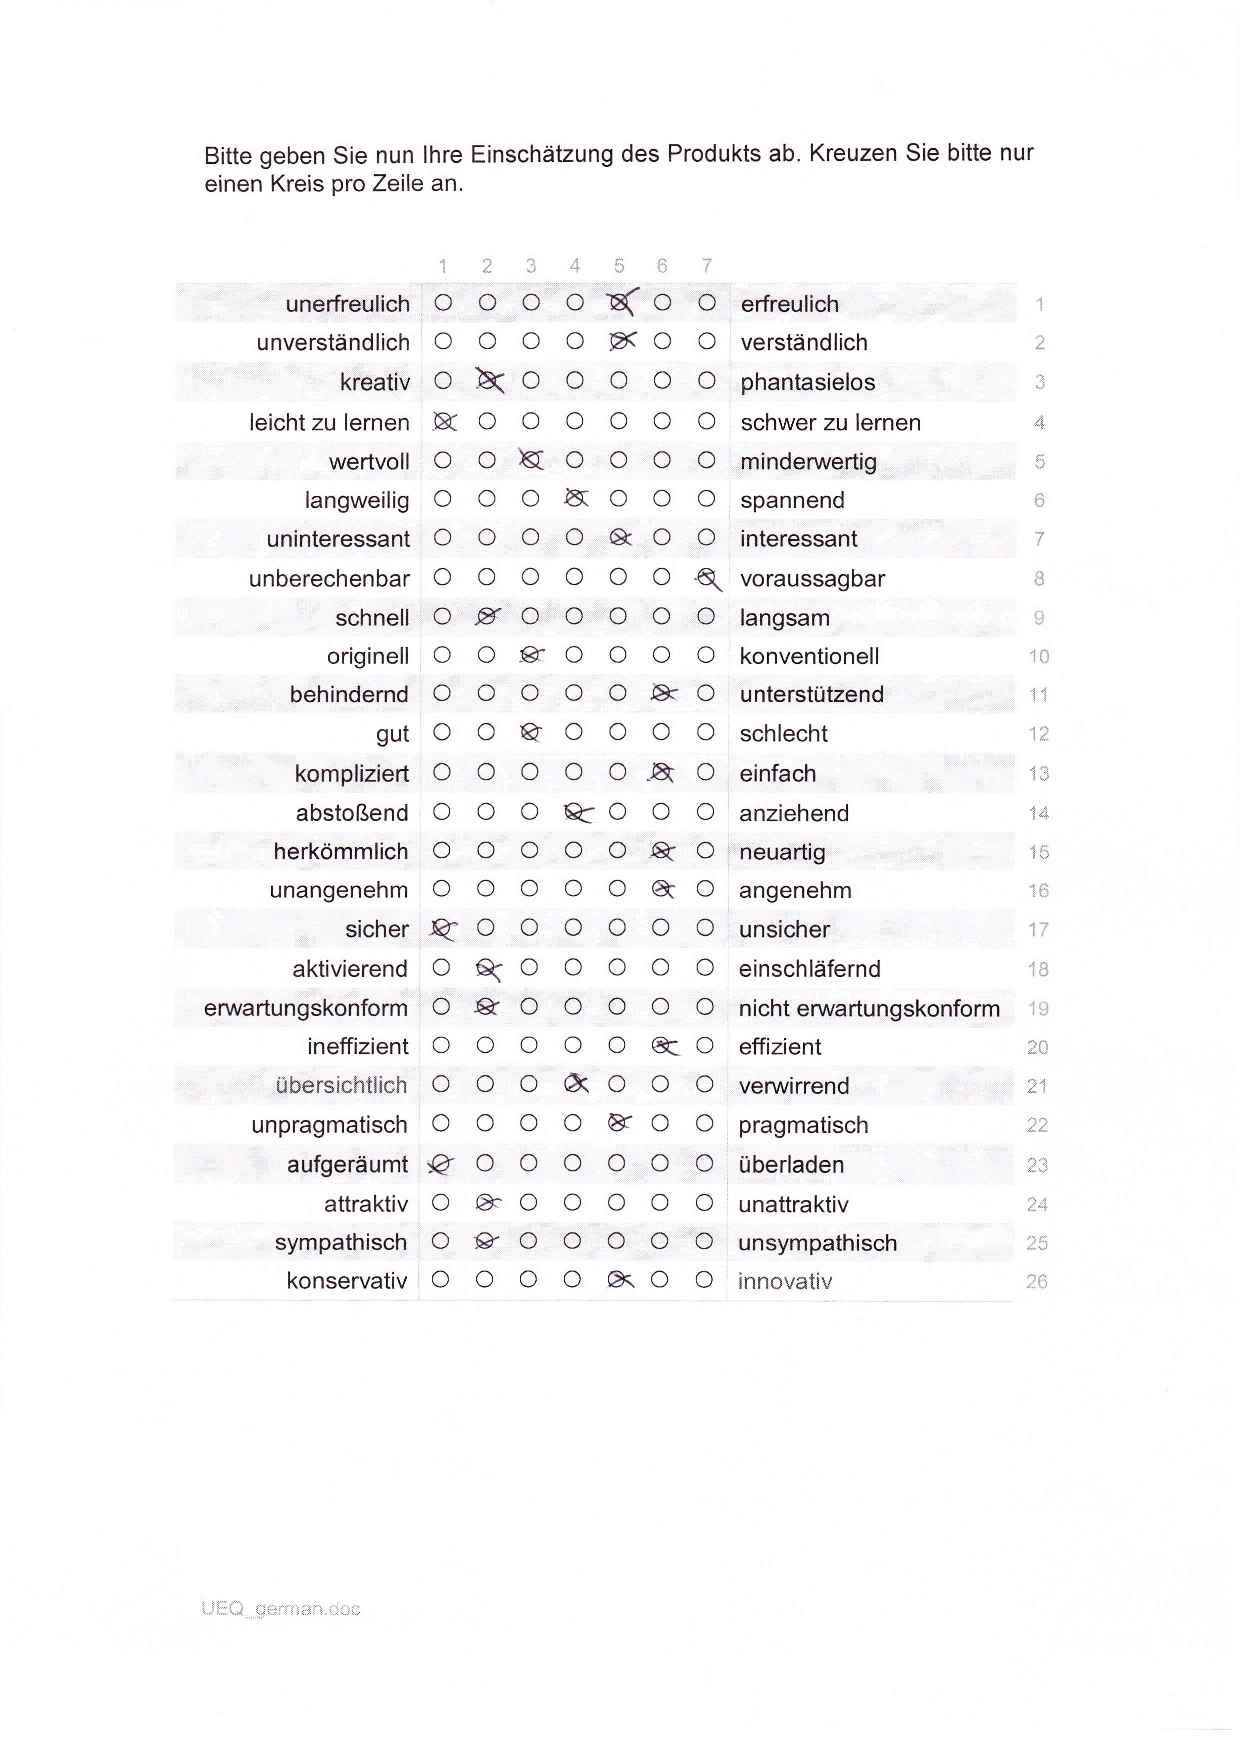
\includegraphics[width=0.85\textwidth,center]{UEQ1.pdf}
\caption{\label{fig:UEQ1}Fragebogen 1}
\end{figure}
\begin{figure}[h!]
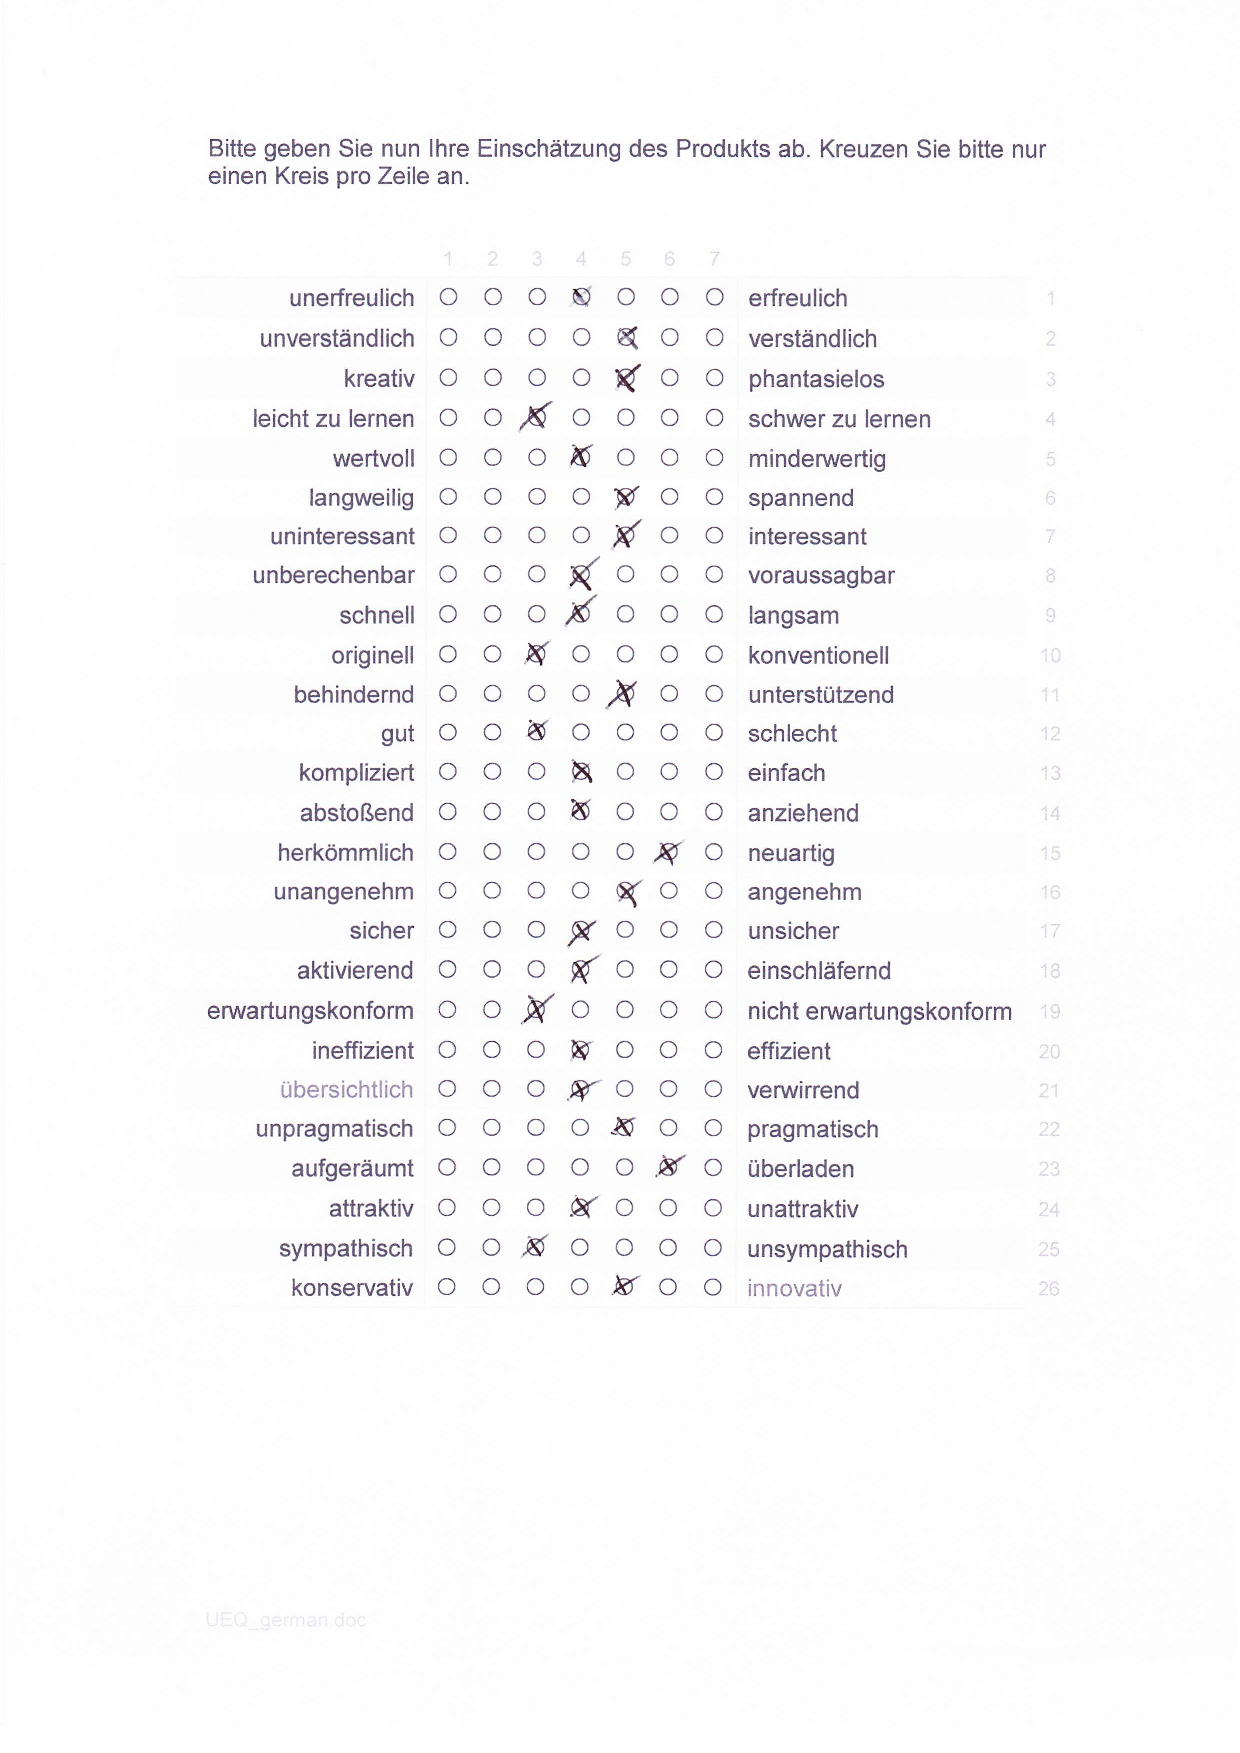
\includegraphics[width=0.85\textwidth,center]{UEQ2.pdf}
\caption{\label{fig:UEQ2}Fragebogen 2}
\end{figure}
\begin{figure}[h!]
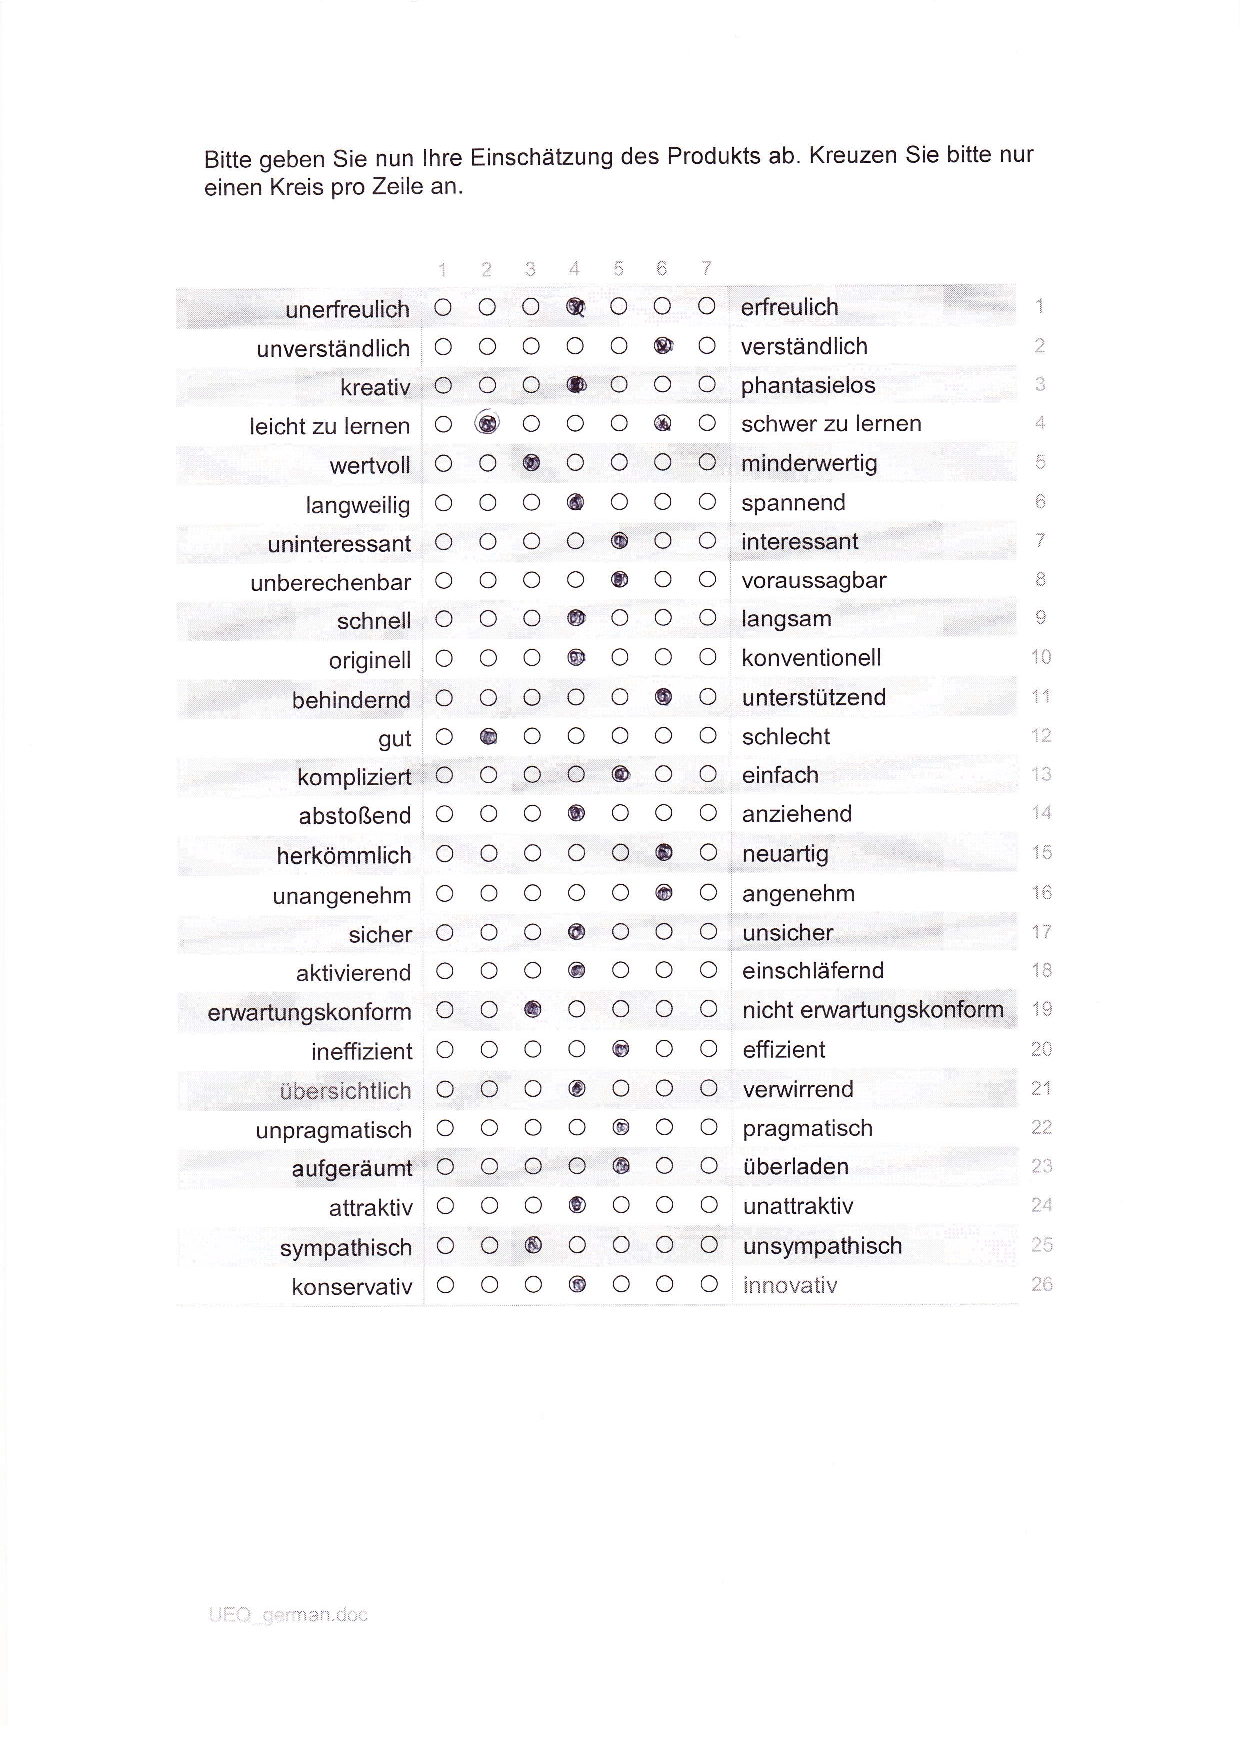
\includegraphics[width=0.85\textwidth,center]{UEQ3.pdf}
\caption{\label{fig:UEQ3}Fragebogen 3}
\end{figure}
\begin{figure}[h!]
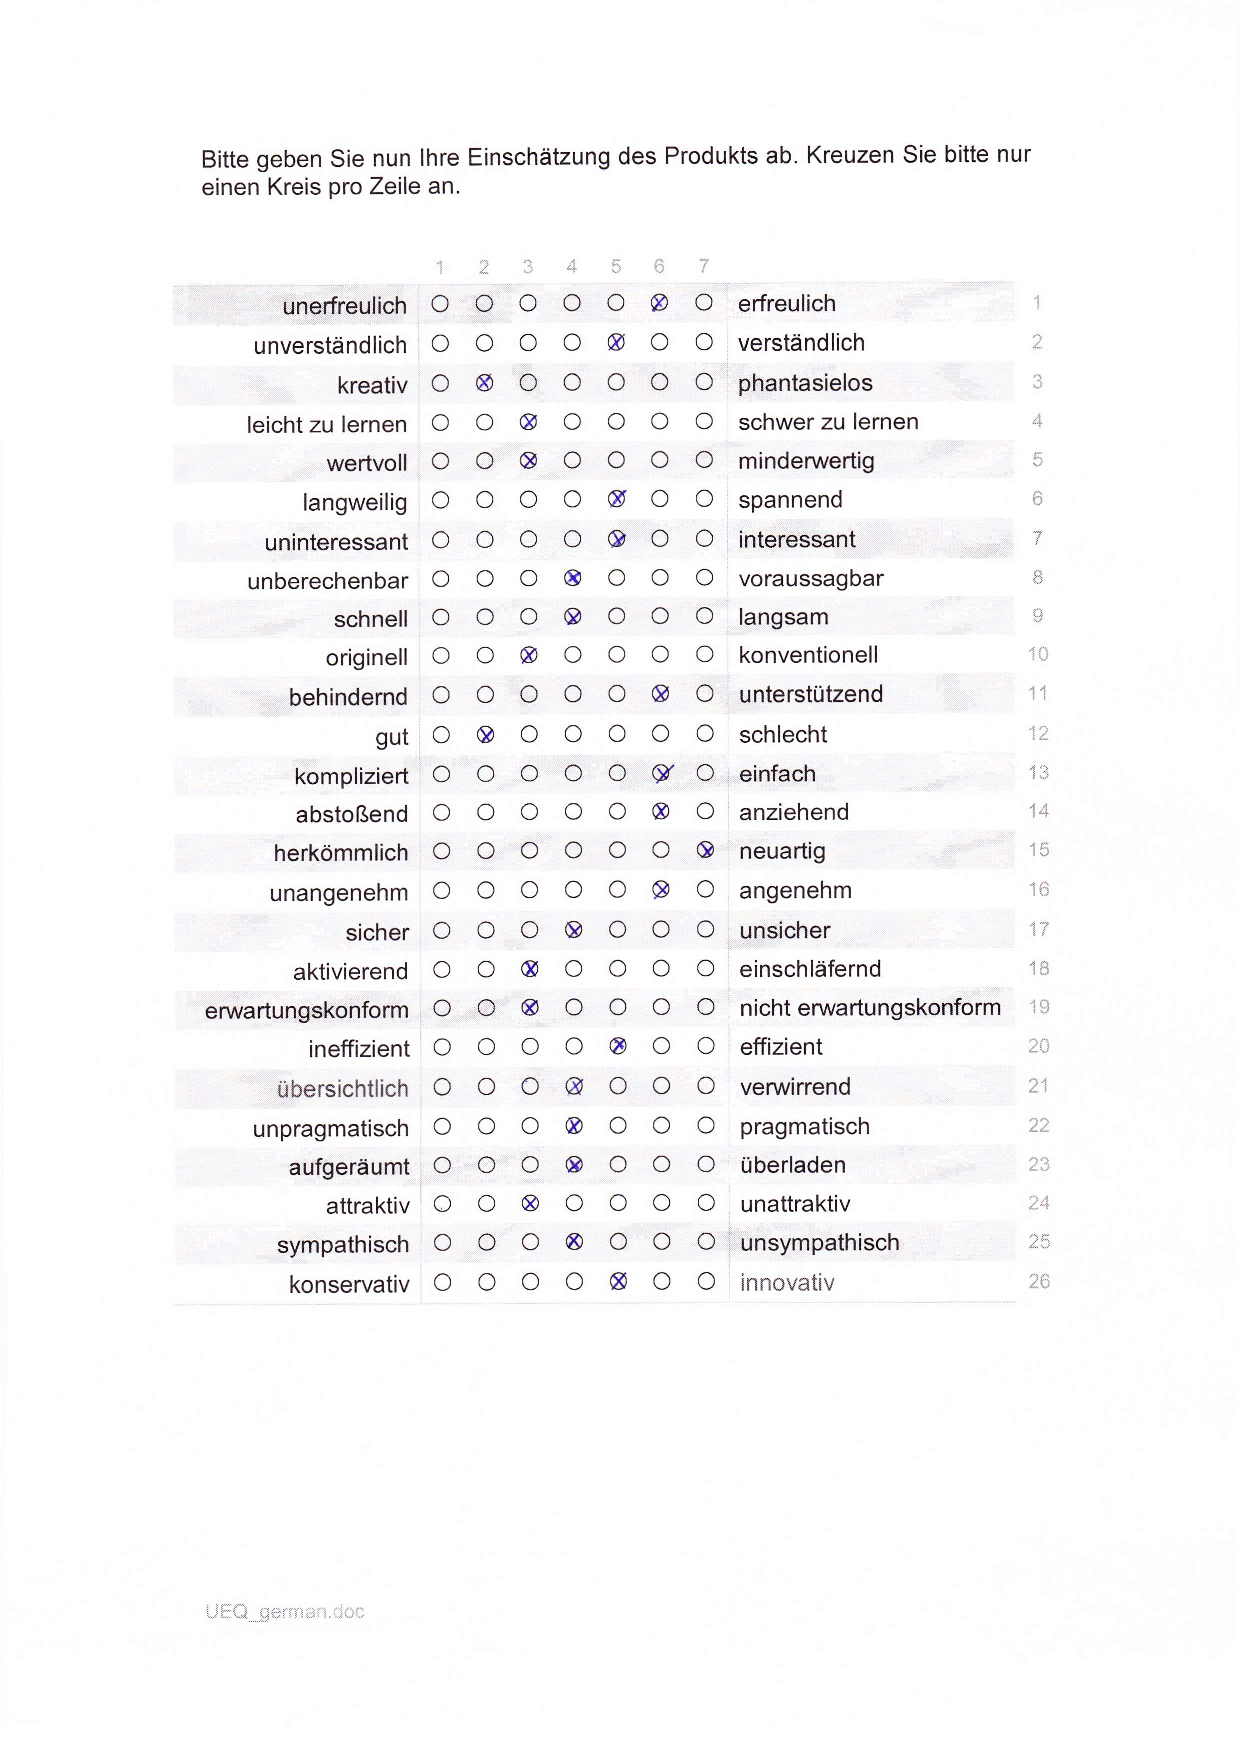
\includegraphics[width=0.85\textwidth,center]{UEQ4.pdf}
\caption{\label{fig:UEQ4}Fragebogen 4}
\end{figure}
\begin{figure}[h!]
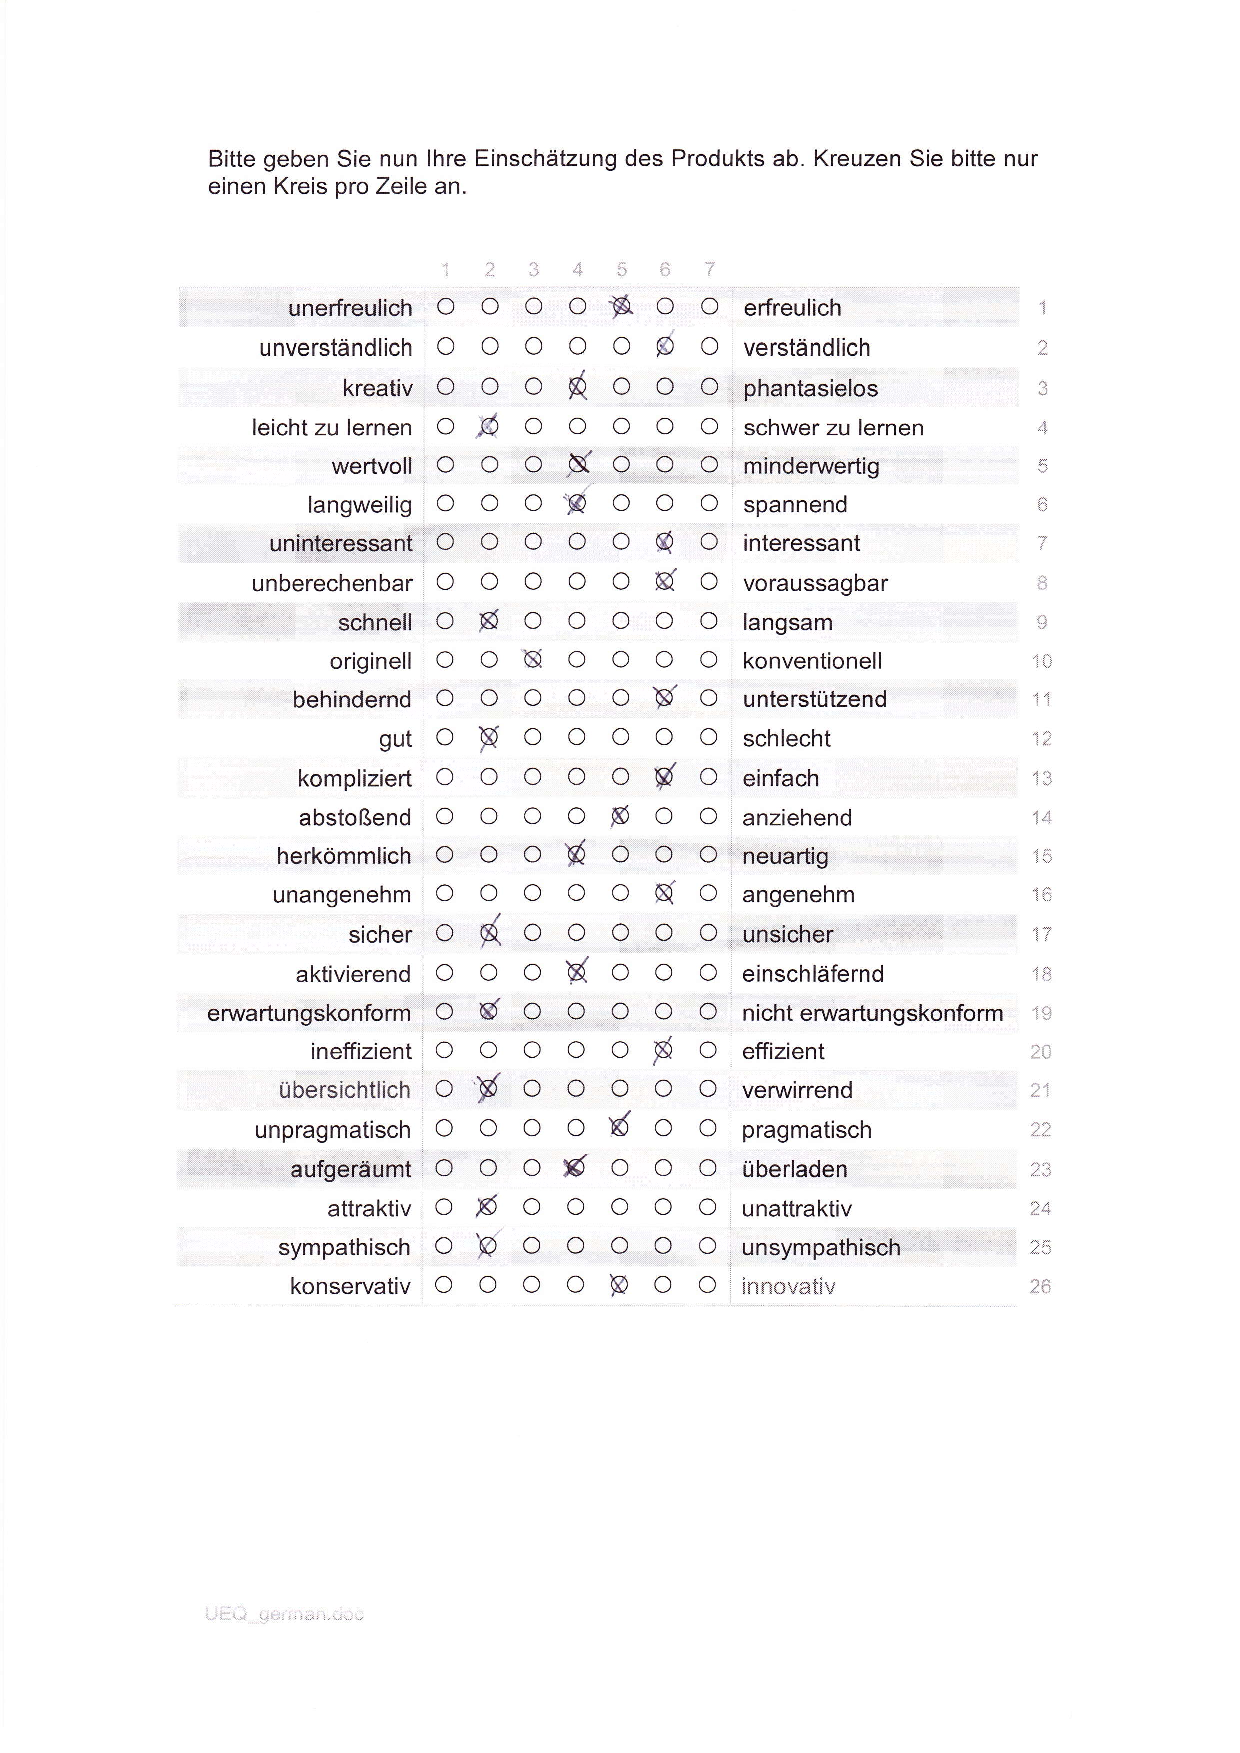
\includegraphics[width=0.85\textwidth,center]{UEQ5.pdf}
\caption{\label{fig:UEQ5}Fragebogen 5}
\end{figure}

